% Created 2020-09-30 Wed 15:22
% Intended LaTeX compiler: pdflatex
\documentclass[10pt,t]{beamer}
\usepackage[utf8]{inputenc}
\usepackage{graphicx}
\usepackage{grffile}
\usepackage{longtable}
\usepackage{wrapfig}
\usepackage{rotating}
\usepackage{textcomp}
\usepackage{amssymb}
\usepackage{capt-of}
\usepackage{hyperref}
\usetheme{default}
%
\usepackage[font=small,labelfont=bf]{caption} % Required for specifying captions
%
\author{C. L. Hepplewhite}
\date{\today}
\title{\large Radiative Transfer Algorithm Updates}
\subtitle{\footnotesize{AIRS Virtual Science Team Meeting}}
\date{\vspace{0.1in}\footnotesize{October 2020 \vfill}}
\author{C. L. Hepplewhite\inst{1,2}, L. Larrabee Strow\inst{1,2}, and S. deSouza Machado\inst{1,2} }
\institute[UMBC]{\inst{1} UMBC Physics Dept. \and \inst{2}UMBC JCET}
\input beamer_setup
\metroset{titleformat title=allcaps}
\setbeamertemplate{frame footer}{UMBC Atmospheric Spectroscopy Lab}
\begin{document}

\maketitle

% -----------------------------------------------------
\begin{frame}{Summary}
\begin{itemize}
  \item What is the Stand-alone radiative transfer algorithm (SARTA)
  \item Who uses SARTA.
  \item Current SARTA build status.
  \item Plans.
    
\end{itemize}

\end{frame}
% -----------------------------------------------------
\begin{frame}{The SARTA}

  \begin{itemize}
  \item The Stand-alone radiative transfer algorithm (SARTA) is constructed using kCARTA
  \item Therefore SARTA has the same spectroscopy as kCARTA.
  \item SARTA was developed 18 years ago for the AIRS.
  \item It uses sets of coefficients that parameterize atmospheric transmittances derived using a set of training profiles.
  \item Is written in Fortran
  \item Permits very fast computation of radiances for predefined spectral response functions.
    \item Has a version for clear sky radiance calculations and for cloudy radiances.
    
\end{itemize}

\end{frame}
% ----------------------------------------------------
\begin{frame}{Who uses SARTA}

  \begin{itemize}
  \item SARTA is used to compute clear and all-sky radiances for any and all FoVs from AIRS, CrIS and IASI missions.
  \item Is fast enough to make whole-mission modelling easily manageable. Faster than kCARTA *way* faster than LBL.
  \item Currently used in ASL for the RTP production for analysis of sensor performance and global studies and geophysical retireval.
  \item Is used in the AIRS geophysical product retrieval.
    \item Is used in NUCAPS.

  \end{itemize}
\end{frame}
% ----------------------------------------------------
\begin{frame}{Current Spectroscopy}

  \begin{itemize}
  \item HITRAN 2016
  \item CO2, CH4 line mixing from LBLRTM12.8
  \item MT CKD3.2
  \item CO2 CIA from WV and N2 by Hartmann (4.3 um)
  \item Single parameter surface emissivity.
    

  \end{itemize}
\end{frame}
% ---------------------------------------------------
\begin{frame}{Possible Future Improvements}

  \begin{itemize}
  \item HITRAN 2020,
  \item Line Mixing package from the HITRAN folks (Iouli Gordon)
  \item Currently use kCARTA at 0.0025 cm-1, can update to 0.0005 cm-1 in 15 um region
  \item poss. linear-in-tau RT.
  \item poss. Nalli surface emissivity parameterization.
    \item poss. look into running off NLTE from Manuel esp. the extreme solar angles
      
  \end{itemize}
\end{frame}

% -------------------------------------------------
\begin{frame}{Current SARTAs at ASL}

  \begin{itemize}
  \item The following SARTAs are in use at ASL:
    \begin{itemize}
    \item AIRS vL1B (2008) as supplied to JPL.
    \item AIRS vL1C (2016).
    \item CrIS NSR v2008, \& v2016.
    \item CrIS FSR v2016
    \item IASI v2008 and v2016.
    \item CHIRP v2016 (under test).
    \end{itemize}
  \end{itemize}
  

\end{frame}
% ------------------------------------------------
\begin{frame}{Validating by bias and residual}

  \begin{itemize}
  \item After completing the fast coefficient regression, top-of-atmosphere (TOA) radiances predicted by SARTA are compared to those from kCARTA from the training set or extended profile set.
  \end{itemize}
      \begin{center}
    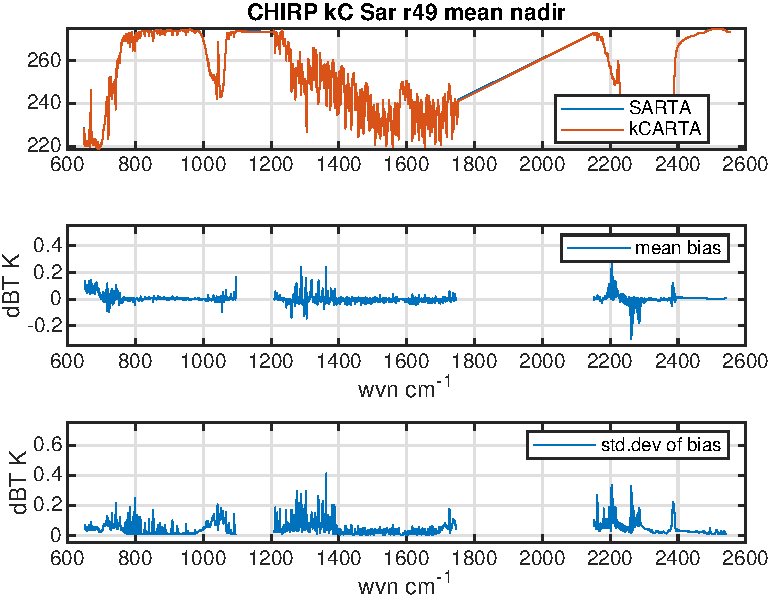
\includegraphics[width=0.6\linewidth]{./Figs/chirp_49regr_sar_kc_bias_stdv.pdf}
    \captionof{figure}{CHIRP channels. AIRS bias relative to SNPP from global statistics. Showing AIRS module bands.}
  \end{center}
  

\end{frame}
% -----------------------------------------------
\begin{frame}{Example of optimization}

\begin{block}{}
  \begin{center}
    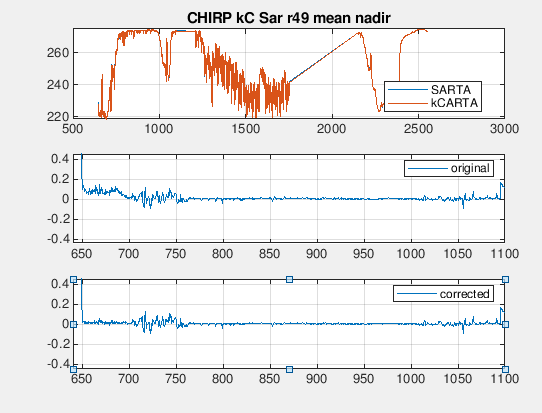
\includegraphics[width=0.6\linewidth]{./Figs/chirp_optimize1.png}
    \captionof{figure}{CHIRP SARTA bias compared to kCARTA, with and without improved regression.}
  \end{center}
\end{block}


\end{frame}
% -----------------------------------------------
\end{document}
